\documentclass{beamer}
\usetheme{metropolis}

\usetheme{metropolis}
\usepackage{listings}

\lstdefinestyle{Python}
{
    language=Python,
    basicstyle=\ttfamily\scriptsize,
    keywordstyle=\color{blue}\ttfamily,
	otherkeywords={self,False},
    commentstyle=\color{green!60!black}\ttfamily,
    stringstyle=\color{red!80!black}\ttfamily,
    backgroundcolor=\color{blue!10!white},
    showstringspaces=false,
    numbers=none,
    numberstyle=\tiny,
    numbersep=5pt,
    xleftmargin=2pt,
    framexleftmargin=4pt,
    framexrightmargin=4pt,
    framexbottommargin=5pt,
    framextopmargin=5pt,
    %breaklines=true,
    captionpos=b
}

\lstdefinestyle{MATLAB}{
    language=MATLAB,
    basicstyle=\ttfamily\scriptsize,
    keywordstyle=\color{blue}\ttfamily,
    stringstyle=\color{red!80!black}\ttfamily,
    commentstyle=\color{green!60!black}\ttfamily,
    numbers=none,
    backgroundcolor=\color{orange!15!white},
    showstringspaces=false,
    numbers=none,
    numberstyle=\tiny,
    numbersep=5pt,
    xleftmargin=2pt,
    framexleftmargin=4pt,
    framexrightmargin=4pt,
    framexbottommargin=5pt,
    framextopmargin=5pt,
    %breaklines=true,
    captionpos=b
}

\renewcommand{\emph}[1]{{\color{red}#1}}

\beamerdefaultoverlayspecification{<+->}

\setbeamercolor{block body}{bg=mDarkTeal!30}
\setbeamercolor{block title}{bg=mDarkTeal,fg=black!2}

\title{Test-Driven Development}
\author{Joachim Vandekerckhove}
\date{}


\newcommand{\module}[1]{{\color{brown}\texttt{#1}}}
\newcommand{\code}[1]{{\color{blue}\texttt{#1}}}

\title{Simulation}
\author{Joachim Vandekerckhove}
\date{}

\usepackage{graphicx}
\begin{document}


\title{Static versus instance methods}
\begin{frame}
  \maketitle
\end{frame}

\begin{frame}[fragile]{Static Methods}
    A static method is a method that \emph{belongs to the class itself} rather than to a particular instance of the class. Here's an example of how to define a static method in Python:
    \begin{lstlisting}[style=python]
    class MyClass:
        @staticmethod
        def my_static_method(arg1, arg2):
            # Code for static method goes here
    \end{lstlisting}
    To call a static method in Python, you can use the class name followed by the method name, like this:
    \begin{lstlisting}[style=python]
    MyClass.my_static_method(arg1, arg2)
    \end{lstlisting}
\end{frame}

\begin{frame}[fragile]{When to Use Static Methods}
    Static methods are useful:
    \begin{itemize}
        \item When a method doesn't need to access any instance variables or methods of the class
        \item When a method needs to be called from both the class and instances of the class
        \item When a method is not logically tied to any particular instance of the class
        \item To create specialized instances of the class
    \end{itemize}
\end{frame}

\begin{frame}[fragile]{Implementation of Static Methods in Python}
    Under the hood, a static method in Python is just a regular function that's defined inside a class. The \code{@staticmethod} decorator is shorthand for this:
    \begin{lstlisting}[style=python]
    class MyClass:
        def my_static_method(arg1, arg2):
            # Code for static method goes here
        my_static_method = staticmethod(my_static_method)
    \end{lstlisting}
    Static methods cannot access instance variables or methods, since they don't have access to a particular instance of the class. If you need to access instance variables or methods, use a regular instance method instead.
\end{frame}

\begin{frame}[fragile]{Static Factory Method}
    A static factory method creates an instance:
    \begin{lstlisting}[style=python]
    class BankAccount:
        def deposit(self, amount):
            self.balance += amount
            
        @staticmethod
        def create_empty():
            return BankAccount(0)
        
        @staticmethod
        def load(filename):
            import pickle
            with open(filename, "rb") as f:
                account = pickle.load(f)
            return account
    
    \end{lstlisting}
    Now you can create basic instances of \code{BankAccount}:
    \begin{lstlisting}[style=python]
    account = BankAccount.create_empty()
    \end{lstlisting}
\end{frame}






\title{Simulation}
\begin{frame}
  \maketitle
\end{frame}

\begin{frame}[fragile]{Random Number Generation: Overview of Algorithms}
    Random number generation is the process of generating a sequence of numbers that are not predictable and have no discernible pattern. There are many algorithms for generating random numbers, but they can be broadly classified into two categories:
    \begin{itemize}
        \item Pseudorandom number generators: These are algorithms that use a deterministic process to generate a sequence of numbers that appear random, but are actually predictable if you know the algorithm and the seed value that was used to initialize it.
        \item True random number generators: These are algorithms that generate numbers from a source of entropy, such as atmospheric noise or radioactive decay, that are truly random and not predictable.
    \end{itemize}
\end{frame}

\begin{frame}[fragile]{Generating Random Numbers in Python}

The \module{numpy} package provides a convenient and efficient way to generate random numbers.

The \code{rand()} function in \module{numpy} generates a random float between 0 and 1.

\begin{lstlisting}[style=python]
import numpy as np

n = np.random.rand()
print(n)  # prints a random float between 0 and 1
\end{lstlisting}

\end{frame}

\begin{frame}[fragile]{Seeding Random Number Generators}
    Pseudorandom number generators use a \emph{seed value} to initialize the algorithm. If you use the same seed value, you will get the same sequence of numbers every time:

\begin{lstlisting}[style=python]
np.random.seed(1234)  # seed with a fixed value
n = np.random.rand()
print(n)  # prints 0.1915194503788923
\end{lstlisting}

By using the same seed value, we can ensure that the same random sequence is generated every time the code is run.

\end{frame}

\begin{frame}[fragile]{Sampling from Statistical Distributions}
The \code{normal()} function in \module{numpy} generates random variables from a Gaussian distribution with the specified mean and standard deviation:

\begin{lstlisting}[style=python]
mu    = 0  # Gaussian mean
sigma = 1  # Gaussian standard deviation

n = np.random.normal(mu, sigma)
\end{lstlisting}

\end{frame}


\begin{frame}[fragile]{More examples}

Generate a sequence of 5 random integers from a binomial distribution with 10 trials and probability of success 0.5
    \begin{lstlisting}[style=python]
b = np.random.binomial(n=10, p=0.5, size=5)
    \end{lstlisting}

Generate 10 numbers from a standard uniform distribution
    \begin{lstlisting}[style=python]
n = np.random.rand(10)
    \end{lstlisting}

Generate 10 integers from a discrete uniform between 1 and 100
    \begin{lstlisting}[style=python]
du = np.random.randint(1, 101, size=10)
    \end{lstlisting}
    
Generate SDT data from 100 signal and 10 noise trials
    \begin{lstlisting}[style=python]
hr, far, nSig, nNoi = .6, .4, 100, 10
hits, fas = np.random.binomial(n=[nSig, nNoi], p=[hr, far])
    \end{lstlisting}

\end{frame}






\begin{frame}{Diffusion Model Sampling}
The diffusion model is a popular cognitive model that describes decision-making processes. In this model, decision-making is represented as a diffusion process of evidence accumulation.

The model assumes that a decision is made by accumulating evidence in favor of one of two alternatives, and that the evidence is accumulated continuously over time until a decision boundary is reached.
\end{frame}


\begin{frame}{Diffusion Model Sampling}
\begin{figure}[htp]
\centering
\includegraphics[scale=0.7]{wdm.eps}
\caption{The Wiener diffusion model}
\label{}
\end{figure}
\end{frame}


\begin{frame}{Euler-Maruyama Method}

\textbf{Idea:} Approximate the continuous-time process $X(t)$ using a discrete-time approximation $X_n = X(n \Delta t)$, where $\Delta t$ is the time step size.

\pause

\begin{block}{Euler-Maruyama Method}
    Given the SDE: 
    $$ dX(t) = f(X(t), t) dt + g(X(t), t) dW(t), $$
    with $X(0) = x_0$, the Euler-Maruyama method generates a numerical approximation $X_n$ for $X(n\Delta t)$ via the recursion: 
    $$ X_{n+1} = X_n + f(X_n, n\Delta t) \Delta t + g(X_n, n\Delta t) \Delta W_n,$$
    where $\Delta W_n = W_{(n+1)\Delta t} - W_{n\Delta t}$ and $W_t$ is the Wiener process.
\end{block}

\end{frame}



\begin{frame}{Diffusion Model Sampling}

To simulate the diffusion process, we can use the following equations:
\begin{align*}
dx_t &= \delta dt + \sigma dW_t \\
x_t &= x_{t-1} + dx_t
\end{align*}

where $x_t$ is the evidence at time $t$, $\delta$ is the drift rate, $\sigma$ is the diffusion coefficient, $dW_t$ is a Wiener process (i.e., a random noise process), and $dt$ is a small time step.

\end{frame}



\begin{frame}[fragile]{Diffusion Model Sampling}

Simulate the diffusion process using \module{numpy}:

\begin{lstlisting}[style=python]
dt, T, mu, sigma, y0 = 0.001, 1.0, 0.1, 0.5, 0.0

# Initialize arrays
t = np.arange(0, T, dt)
y = np.zeros_like(t) + y0

# Simulate diffusion process
for i in range(1, len(t)):
    dy = mu * dt + sigma * np.sqrt(dt) * np.random.randn()
    y[i] = y[i-1] + dy

\end{lstlisting}

\end{frame}


\begin{frame}[fragile]{Diffusion Model Sampling}
\begin{figure}[htp]
\centering
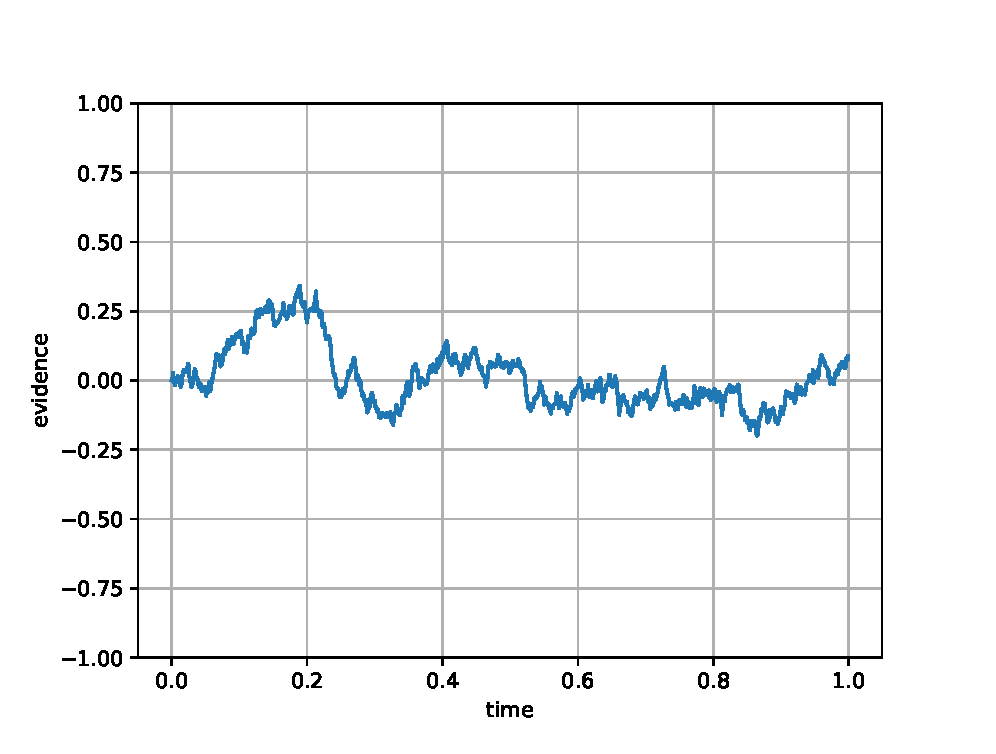
\includegraphics[scale=0.55]{pydiff.eps}
\caption{A single diffusion process}
\label{}
\end{figure}
\end{frame}





\end{document}

% Static methods
% Random number generation
% - Streams
% Simulating data


% HW:
% - Simulate SDT data
% - ROC Curve
% - Fit ROC curve?
% - Fit line?